\chapter{Introduction} \label{ch:introduction}

From the Vedas to the ancient Greeks, generations have described the constituents of nature in terms of indivisible `elements'.  It wasn't until the modern era that the ancient elements of earth, wind, fire, and water were abandoned for the atomic theory of nature.  By the 1960's, what would become known as the Standard Model of Particle Physics was taking shape.  The four ancient elements were replaced by the two fundamental particles types: the mass carrying fermions with spin 1/2, and the force carrying bosons with spin 1, as seen in Figure \ref{fig:fundpart}.


\begin{figure}[h]
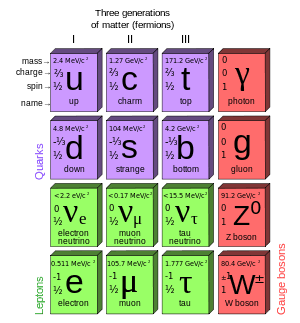
\includegraphics[width=6.0cm]{Fundamental_Particles}
\centering
\caption{The fundamental particles of the Standard Model\cite{Patrignani:2016xqp}.}
\label{fig:fundpart}
\end{figure}


\par
The Standard Model is the unification of the three symmetry groups, SU(3) x SU(2) x U(1), representing the strong, weak, and electromagnetic forces respectively\cite{Langacker:2009my}.  In terms of scientific accomplishments, the Standard Model is one of the most tested theories of nature with an agreement between the theory and observed results up to ten digits\cite{Aoyama:2014sxa}.  Even though the Standard Model gives us a deep understanding of many natural phenomena and has a wide range of uses, from understanding the evolution of the Big Bang, the bonding of atoms and molecules, and the nature of light, to cancer treatments and nuclear security, it is fundamentally an incomplete theory of nature.  The fact that Gravity has yet to be unified into a quantum theory tells us that the Standard Model is incomplete.  High energy experiments give us some of the most extreme conditions possible to test the Standard Model and to look for phenomena outside of the theory.  Are there new symmetries and laws that manifest at high energies? Can we create dark matter or dark energy in a laboratory?  Are quarks and leptons fundamental or finite in size?  Do the four fundamental forces emerge from some yet unknown unified force?  And why is antimatter absent in the Universe?  All of these open questions are of great interest and currently form large areas of active research.  

\par
The theory of strong interactions, Quantum Chromodynamics QCD is described by the SU(3) group and is analogous to Quantum Electrodynamics (QED) with gluons being the force mediator instead of photons and quarks carrying mass.  Quarks and gluons are known as partons and are particles that interact via the strong force.  At low energies and over large length scales, partons are confined to a color neutral state and they must clump together into color neutral hadrons.  As two colored partons begin to separate, at some point it becomes energetically favorable to create a quark--antiquark pair out of the vacuum rather then expanding the distance between neighboring partons.  Due to confinement, high energy scatterings between two partons will lead to a spray of hadrons known as a `jet'.  The other main attribute of QCD is asymptotic freedom, as the interactions between partons become more energetic and the length scale decreases, the strong coupling constant becomes exceedingly small, $ \alpha_{strong} << 1$, and the partons freely interact with one another.  Due to asymptotic freedom, nuclear matter undergoes a phase transition called the Quark--Gluon Plasma (QGP) at high energies and densities. 

\par
The analysis performed during this thesis explored jet production and kinematics in proton-proton collisons at the Large Hadron Collider.  It will also report constraints on the different mechanisms involved in jet production and help serve as a baseline for jet measurements in heavy-ion collisions.

This thesis will present an overview of QCD in Chapter \ref{ch:qcd}, with an emphasis on jet physics and heavy ion collisions.  Chapter \ref{ch:alice} will give a brief overview of the LHC and the ALICE experiment, including the relevant subsystems for this thesis.  Chapter \ref{ch:tpcu} will discuss the contribution to the upgrade of the ALICE Time Projection Chamber performed during my Ph.D. studies.  A discussion of quality control and assureance performed on the data collected from ALICE isgiven in Chapter \ref{ch:data}.  Chapter \ref{ch:error} will discuss the analysis corrections and systematic error calculations.  Finally, Chapter \ref{ch:cando} will present the final fully corrected results and give an outlook on the analysis. 